

%\newcommand{\statartscount}{$900,901$}
%\newcommand{\statmavensize}{$1.7$ TB}
%\newcommand{\statuniqueartscount}{$100,885$}
%\newcommand{\statrepouniquearts}{$75,405$}
%\newcommand{\statreposize}{$70$ GB}
%\newcommand{\statdeponunsafe}{$25\%$}

%\newcommand{\statunsafeuses}{$40,343$}
%\newcommand{\statunsafecs}{$40,040$}
%\newcommand{\statunsafefieldusages}{$303$}
%\newcommand{\statunsafearts}{$720$}

%\newcommand{\statartwithpominfo}{$40,622$}
%\newcommand{\statartsdepuns}{$19,333$}
%\newcommand{\statpercartsdepunsovertotal}{47\%}
%\newcommand{\statpercartsdepunsoverpominfo}{25\%}


\newcommand{\statartscount}{$959,300$}
\newcommand{\statmavensize}{$1.7$ TB}
\newcommand{\statuniqueartscount}{$106,574$}
\newcommand{\statrepouniquearts}{$86,479$}
\newcommand{\statreposize}{$74$ GB}
\newcommand{\statdeponunsafe}{$25\%$}

\newcommand{\statunsafeuses}{$48,490$}
\newcommand{\statunsafecs}{$48,139$}
\newcommand{\statunsafefieldusages}{$351$}
\newcommand{\statunsafearts}{$817$}

\newcommand{\statartswithpominfo}{$47,127$}

\newcommand{\statartsdepuns}{$21,297$}
\newcommand{\statpercartsdepunsoverpominfo}{47\%}
\newcommand{\statpercartsdepunsovertotal}{25\%}

\newcommand{\statartsdepunsapp}{$19,173$}
\newcommand{\statpercartsdepunsoverpominfoapp}{41\%}
\newcommand{\statpercartsdepunsovertotalapp}{22\%}


\definecolor{header-color}{HTML}{D1D1D1}
\definecolor{alt-row-color}{HTML}{ECECEC}

\newcommand{\artstyle}[1]{\textsl{#1}}
\newcommand{\artexp}[2]{\artstyle{#1}:\artstyle{#2}}
\newcommand{\art}[3]{\artstyle{#1}:\artstyle{#2}\footnote{\url{#3}}}

\newcommand{\member}[1]{\emph{#1}}
\newcommand{\smugroup}[1]{\textsl{#1}}
\newcommand{\stackoverflow}{Stack Overflow}

\chapter{The \java{} Unsafe \api{} in the Wild}
\label{cha:unsafe}

The \java{} Virtual Machine (\jvm{}) executes \java{} bytecode and
provides other services for programs written in
many programming languages, including \java{}, \scala{}, and \clojure{}.
The \jvm{} was designed to provide strong safety guarantees.
However, many widely used \jvm{} implementations expose an \api{} that
allows the developer to access low-level,
unsafe features of the \jvm{} and underlying hardware,
features that are unavailable in safe \java{} bytecode.
This \api{} is provided through an undocumented%
\footnote{\url{http://www.oracle.com/technetwork/java/faq-sun-packages-142232.html}}
class, \smu{}, in the \java{} reference implementation produced by Oracle.

Other virtual machines provide similar functionality.
For example, the \csharp{} language provides an \code{unsafe} construct
on the .NET platform,%
\footnote{\url{https://msdn.microsoft.com/en-us/en-en/library/chfa2zb8(v=vs.90).aspx}}
and \racket{} provides unsafe operations.%
\footnote{\url{http://docs.racket-lang.org/reference/unsafe.html}}

The operations \smu{} provides can be dangerous,
as they allow developers to circumvent the safety guarantees provided by
the \java{} language and the \jvm{}.
If misused, the consequences can be resource leaks, deadlocks,
data corruption, and even \jvm{} crashes.%
\footnote{\url{https://groups.google.com/d/msg/elasticsearch/Nh-kXI5J6Ek/WXIZKhhGVHkJ}}
\footnote{\url{https://github.com/EsotericSoftware/kryo/issues/219}}
\footnote{\url{https://github.com/dain/snappy/issues/24}}
\footnote{\url{https://netbeans.org/bugzilla/show_bug.cgi?id=229655}}
\footnote{\url{https://netbeans.org/bugzilla/show_bug.cgi?id=244914}}

We believe that \smu{} was introduced to provide better performance and
more capabilities to the writers of the \java{} runtime library.
However, \smu{} is increasingly being used in third-party
frameworks and libraries.
Application developers who rely on \java{}'s safety guarantees have to
trust the implementers of the language runtime environment
(including the core runtime libraries).
Thus the use of \smu{} in the runtime libraries is no more risky than
the use of an unsafe language to implement the \jvm{}.
However, the fact that more and more ``normal'' libraries are using
\smu{} means that application developers have to trust a growing
community of third-party \java{} library developers to not
inadvertently tamper with the fragile internal state of the \jvm{}.

Given that the benefits of safe languages are well known,
and the risks of unsafe languages are obvious,
why exactly does one need unsafe features in third-party libraries?
Are those features used in real-world code?
If yes, how are they used, and what are they used for?

We studied a large repository of \java{} code, \mavencentral{},
to answer these questions.
We have analyzed \statreposize{} of compiled \java{} code,
spread over \statrepouniquearts{} \java{} archives,
to determine how \java{}'s unsafe capabilities are used in real-world
libraries and applications.
We found that $25\%$ of \java{} bytecode archives depend on unsafe
third-party \java{} code, and thus \java{}'s safety
guarantees cannot be trusted.
We identify $14$ different usage patterns of \java{}'s unsafe capabilities,
and we provide supporting evidence for why real-world code needs these capabilities.
Our long-term goal is to provide a strong foundation
to make informed decisions in the future evolution of the \java{} language and virtual machine,
and for the design of new language features to regain safety in \java{}.

We have already published our work on how developers use the Unsafe \api{} in \java{}~\citep{mastrangeloUseYourOwn2015}.
In this thesis we outline the risks of using the \unsafe{} \api{} in \S\ref{sec:unsafe:background}.
Then we answer \ref{unsafe:rq1} in \S\ref{sec:unsafe:overview}.
To answer \ref{unsafe:rq2}, first we introduce our methodology and the patterns we found in \S\ref{sec:unsafe:methodology} and \S\ref{sec:unsafe:patterns} respectively, to then present how the patterns we found could be implemented in a safer way in \S\ref{sec:unsafe:discussion}.

\section{The Risks of Compromising Safety}
\label{sec:unsafe:background}

We outline the risks of \unsafe{} by illustrating how the improper use of
\unsafe{} violates \java{}'s safety guarantees.

In \java{}, the unsafe capabilities are provided as instance methods of
class \smu{}.
Access to the class has been made less than straightforward.
Class \smu{} is final, and its constructor is not public.
Thus, creating an instance requires some tricks.
For example, one can invoke the private constructor via reflection.
This is not the only way to get hold of an unsafe object,
but it is the most portable.

\begin{lstlisting}[style=java,caption=Instantiating an Unsafe object]
Constructor<Unsafe> c = Unsafe.class.getDeclaredConstructor();
c.setAccessible(true);
Unsafe unsafe = c.newInstance();
\end{lstlisting}
 
Given the unsafe object, one can now simply invoke any of its methods to
directly perform unsafe operations.

\subsection{Violating Type Safety}

In \java{}, variables are strongly typed.
For example, it is impossible to store an int value inside a variable of
a reference type.
\unsafe{} can violate that guarantee:
it can be used to store a value of any type in a field or array element.

\begin{lstlisting}[style=java,caption=\smu{} can violate type safety]
class C {
  private Object f = new Object();
}
long fieldOffset = unsafe.objectFieldOffset(
        C.class.getDeclaredField("f") );
C o = new C();
unsafe.putInt(o, fieldOffset, 1234567890);      // f now points to nirvana
\end{lstlisting}

\subsection{Crashing the Virtual Machine}

A quick way to crash the VM is to free memory that is in a protected
address range, for example by calling \code{freeMemory} as follows.

\begin{lstlisting}[style=java,caption=\smu{} can crash the VM]
unsafe.freeMemory(1);
\end{lstlisting}

In \java{}, the normal behavior of a method to deal with such situations
is to throw an exception.
Being unsafe, instead of throwing an exception,
this invocation of \code{freeMemory} crashes the VM.

\subsection{Violating Method Contracts}

In \java{}, a method that does not declare an exception cannot throw any
checked exceptions.
\unsafe{} can violate that contract:
it can be used to throw a checked exception that the surrounding method
does not declare or catch.

\begin{lstlisting}[style=java,caption=\smu{} can violate a method contract]
void m() {
  unsafe.throwException(new Exception());
}
\end{lstlisting}

\subsection{Uninitialized Objects}

\java{} guarantees that an object allocation also initializes the object
by running its constructor.
\unsafe{} can violate that guarantee:
it can be used to allocate an object without ever running its
constructor.
This can lead to objects in states that the objects' classes would
not seem to admit.

\begin{lstlisting}[style=java,caption=\smu{} can lead to uninitialized objects]
class C {
  private int f;
  public C() { f = 5; }
  public int getF() { return f; }
}

C c = (C)unsafe.allocateInstance(C.class);
assert c.getF()==5; // violated
\end{lstlisting}

\subsection{Monitor Deadlock}

\java{} provides synchronized methods and synchronized blocks.
These constructs guarantee that monitors entered at the beginning
of a section of code are exited at the end.
\unsafe{} can violate that contract:
it can be used to asymmetrically enter or exit a monitor,
and that asymmetry might be not immediately obvious.

\begin{lstlisting}[style=java,caption=\smu{} can lead to monitor deadlocks]
void m() {
  unsafe.monitorEnter(o);
  if (c) return;
  unsafe.monitorExit(o);
}
\end{lstlisting}

The above examples are just the most straightforward violations of
\java{}'s safety guarantees.
The \smu{} class provides a multitude of methods that can be used
to violate most guarantees \java{} provides.

To sum it up: \unsafe{} is dangerous.
But should anybody care?
In the next sections we present a study to determine whether and how
\unsafe{} is used in real-world third-party \java{} libraries,
and to what degree real-world applications directly and indirectly
depend on it.

\section{Is Unsafe Used?}
\label{sec:unsafe:overview}

To answer~\ref{unsafe:rq1} (\emph{\urqA})
we need to determine whether and how Unsafe is actually used in real-world third-party \java{} libraries,
and to what degree real-world applications directly and indirectly depend on such unsafe libraries.
To achieve our goal, several elements are needed.

\textbf{Code Repository.}
As a code base representative of the ``real world'',
we have chosen the Maven Central software repository.
% The rationale behind this decision is that a large number of well-known \java{} projects deploy to Maven Central using Apache Maven.
% Besides code written in \java{}, projects written in \lang{Scala} are also deployed to Maven Central using the Scala Build Tool (sbt).
% Moreover, Maven Central is the largest \java{} repository\footnote{\url{http://www.modulecounts.com/}}
% , and it contains projects from the most popular source code management repositories, like \github{} and \sourceforge{}.

\textbf{Artifacts.}
In Maven, an artifact is the output of the build procedure of a project.
% An artifact can be any type of file, ranging from a \emph{.pdf} to a \emph{.zip} file.
% However,
Artifacts are usually \emph{.jar} files,
which archive compiled \java{} bytecode stored in \emph{.class} files.

\textbf{Bytecode Analysis.}
% We examine these kinds of artifacts to analyze how they use \code{sun.misc.\-Unsafe}.
We use a bytecode analysis library to search for method call sites and field accesses of the \code{sun.misc.Unsafe} class.

\textbf{Dependency Analysis.}
We define the impact of an artifact as how many artifacts depend on it,
either directly or indirectly.
This helps us to define the impact of artifacts that use \code{sun.misc.Unsafe},
and thus the impact \code{sun.misc.Unsafe} has on real-world code overall.

% \textbf{Usage Pattern Detection.}
% After all call sites and field accesses are found,
% we analyze this information to discover usage patterns.
% It is common that an artifact exhibits more than one pattern.
% Our list of patterns is not exhaustive.
% We have manually investigated the source code of the 100 highest-impact artifacts using \code{sun.misc.Unsafe} to understand why and how they are using it.




Our analysis found $48,490$ uses of \code{sun.misc.Unsafe} --- $48,139$ call sites and $351$ field accesses --- distributed over $817$ different artifacts.
This initial result shows that Unsafe is indeed used in third-party code.

We use the dependency information to determine the impact of the artifacts that use \code{sun.misc.Unsafe}.
We rank all artifacts according to their impact (the number of artifacts that directly or indirectly depend on them).
High-impact artifacts are important;
a safety violation in them can affect any artifact that directly or indirectly depends on them.
We find that while overall about $1\%$ of artifacts directly use Unsafe,
for the top-ranked $1000$ artifacts, $3\%$ directly use Unsafe.
Thus, Unsafe usage is particularly prevalent in high-impact artifacts, artifacts that can affect many other artifacts.

Moreover, we found that $21,297$ artifacts ($47\%$ of the $47,127$ artifacts with dependency information, or $25\%$ of the $86,479$ artifacts we downloaded) directly or indirectly depend on \code{sun.misc.Unsafe}.
Excluding language artifacts, numbers do not change much:
Instead of $21,297$ artifacts, we found $19,173$ artifacts,
$41\%$ of the artifacts with dependency information, or $22\%$ of artifacts downloaded.
Thus, \code{sun.misc.Unsafe} usage in third-party code indeed impacts a large fraction of projects.

\subsection*{Which Features of \unsafe{} Are Actually Used?}

\begin{figure}[!ht]
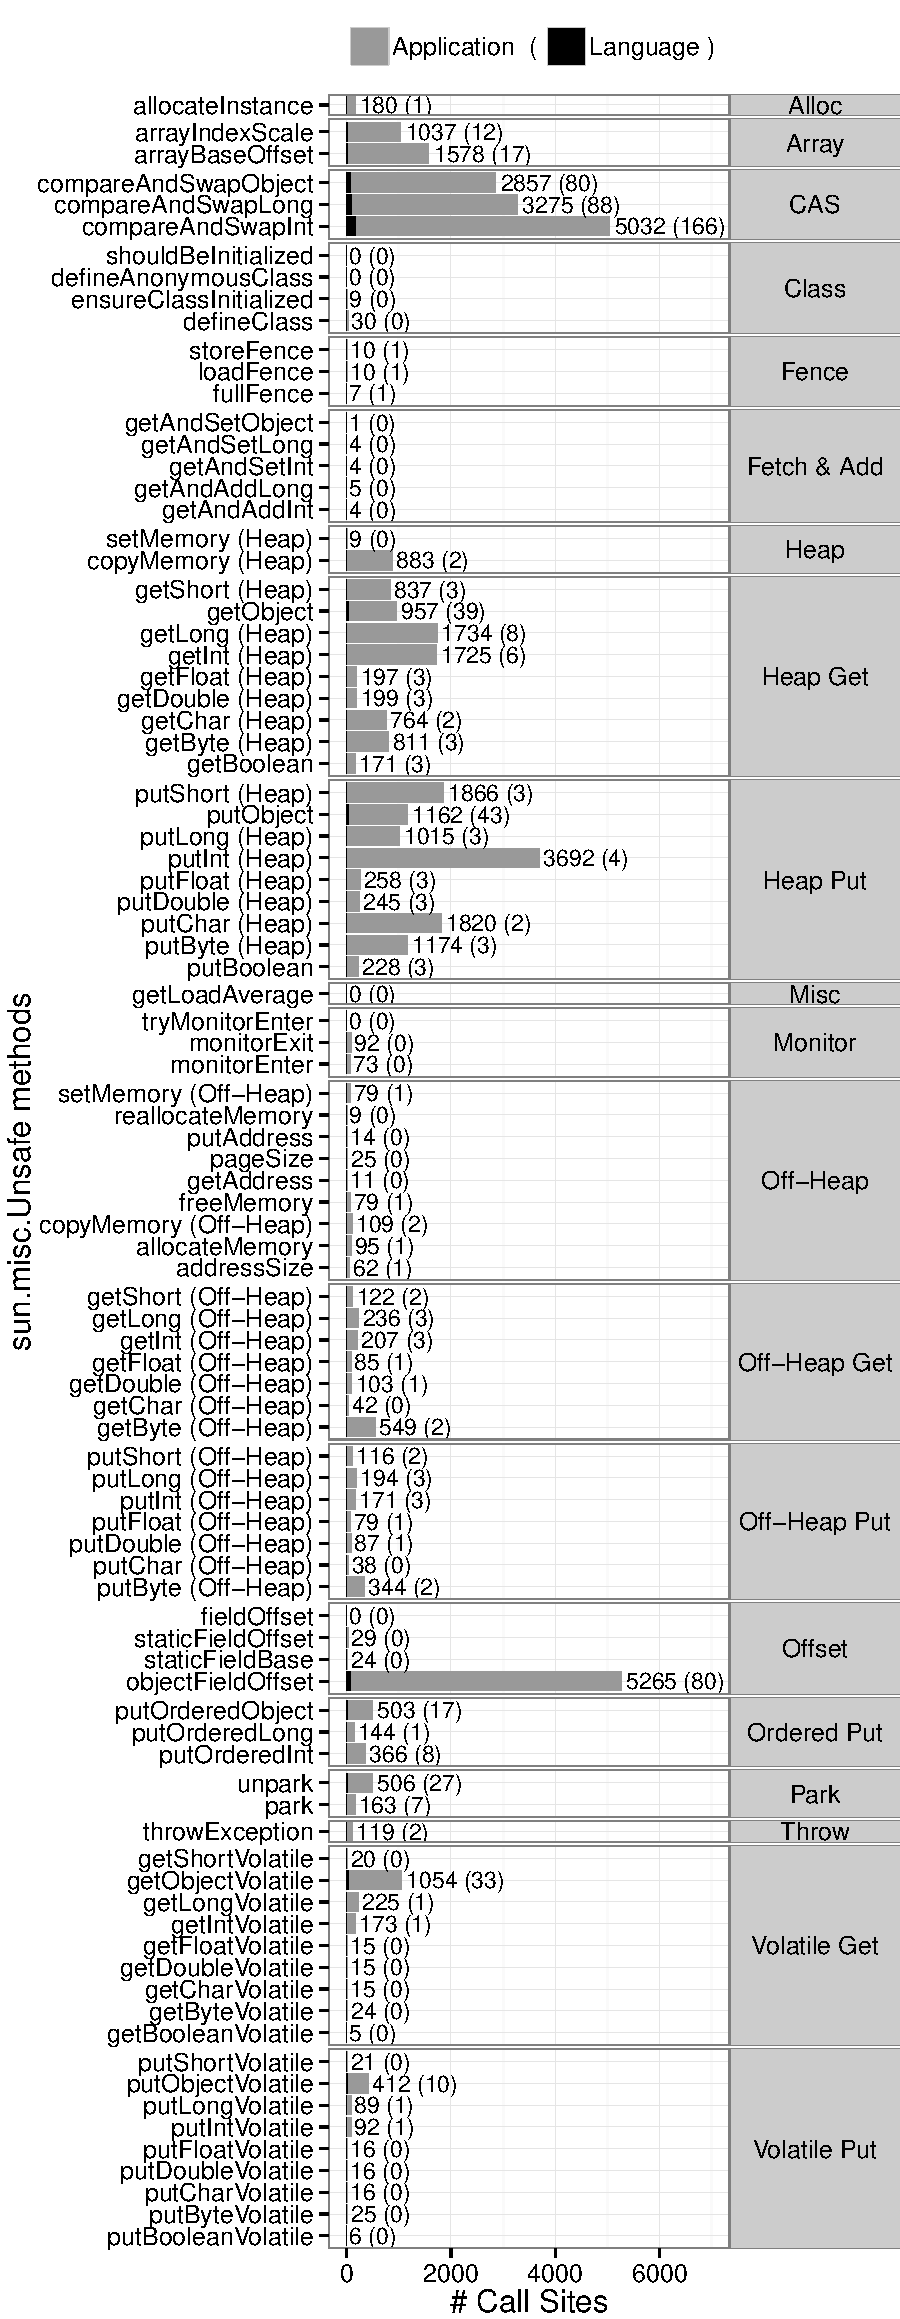
\includegraphics[width=0.5\columnwidth]{chapters/unsafe/usage-maven-methods}
\caption{\smu{} method usage on \mavencentral{}}
\label{fig:overview}
\end{figure}

\begin{figure}[!ht]
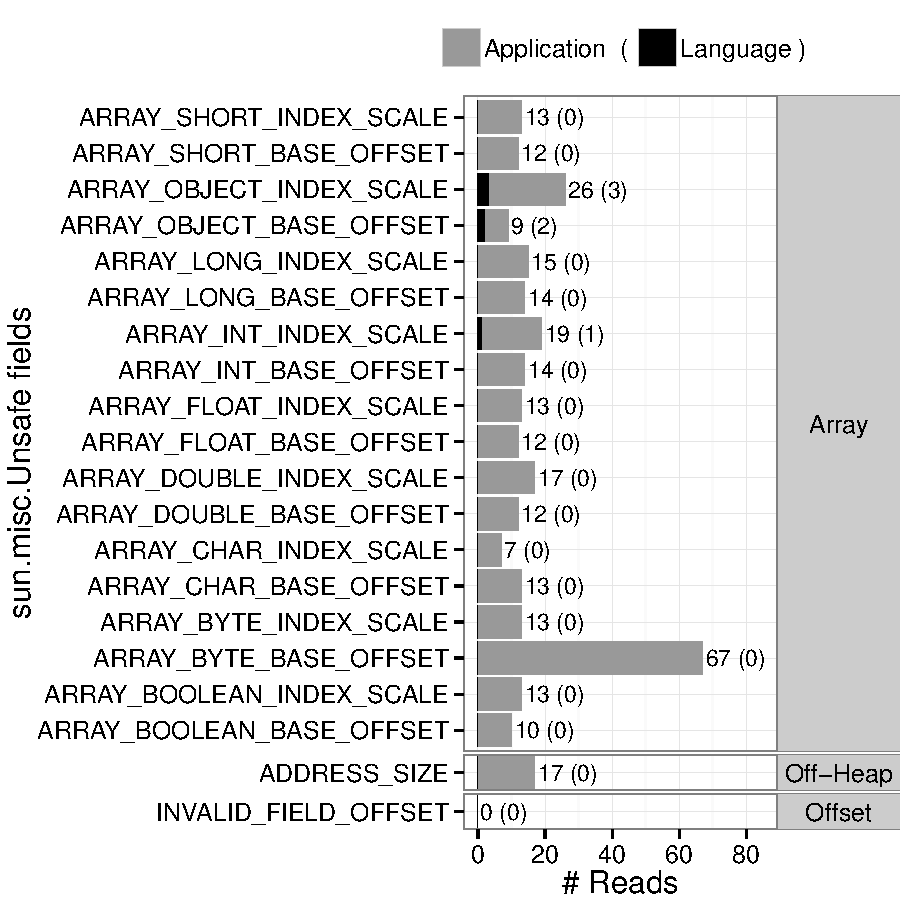
\includegraphics[width=0.7\columnwidth]{chapters/unsafe/usage-maven-fields}
\caption{\smu{} field usage on \mavencentral{}}
\label{fig:overview-field}
\end{figure}

Figures~\ref{fig:overview} and~\ref{fig:overview-field} show all instance methods and static fields of \smu{}. For each member we show how many call sites or field accesses we found across the artifacts. The class provides $120$ public instance methods and $20$ public fields (version 1.8 update 40). The figure only shows $93$ methods because the $18$ methods in the \smugroup{Heap Get} and \smugroup{Heap Put} groups, and \member{staticFieldBase} are overloaded, and we combine overloaded methods into one bar.

We show two columns, \smugroup{Application} and \smugroup{Language}.
The \smugroup{Language} column corresponds to language implementation artifacts while the \smugroup{Application} column corresponds to the rest of the artifacts.

We categorized the members into groups, based on the functionality they provide:

\begin{itemize}
  
\item The \smugroup{Alloc} group contains only the  \member{allocateInstance} method, 
which allows the developer to allocate a \java{} object without executing a constructor.
This method is used 181 times: 180 in \smugroup{Application} and 1 in \smugroup{Language}.

\item The \smugroup{Array} group contains methods and fields for computing relative addresses of array elements.
The fields were added as a simpler and potentially faster alternative in a more recent version of \unsafe{}.
The value of all fields in this group are constants initialized with the result of a call to either \member{arrayBaseOffset} or \member{arrayIndexScale} in the \smugroup{Array} group.
The figures show that the majority of sites still invoke the methods instead of accessing the corresponding constant fields.

\item The \smugroup{CAS} group contains methods to atomically compare-and-swap a \java{} variable. These operations are implemented using processor-specific atomic instructions. For instance, on \emph{x86} architectures, \member{compareAndSwapInt} is implemented using the \texttt{CMPXCHG} machine instruction. Figure~\ref{fig:overview} shows that these methods represent the most heavily used feature of \unsafe{}.

\item Methods of the \smugroup{Class} group are used to dynamically load and check \java{} classes. They are rarely used, with \member{defineClass} being used the most.

\item 
The methods of the \smugroup{Fence} group provide memory fences to ensure loads and stores are visible to other threads.
These methods are implemented using processor-specific instructions.
These methods were introduced only recently in \java{} 8, which explains their limited use in our data set.
We expect that their use will increase over time and that other operations, such as those in the \smugroup{Ordered Put}, or \smugroup{Volatile Put} groups will decrease as programmers use the lower-level fence operations.

\item The \smugroup{Fetch \& Add} group, like the \smugroup{CAS} group, allows the programmer to atomically update a \java{} variable. This group of methods was also added recently in \java{} 8. We expect their use to increase as programmers replace some calls to methods in the \smugroup{CAS} group with the new functionality.

\item The \smugroup{Heap} group methods are used to directly access memory in the \java{} heap. The \smugroup{Heap Get} and \smugroup{Heap Put} groups allow the developer to load and store a Java variable. These groups are among the most frequently used ones in \unsafe{}.

\item The \smugroup{Misc} group contains the method \member{getLoadAverage}, to get the load average in the operating system run queue assigned to the available processors. It is not used.

\item The \smugroup{Monitor} group contains methods to explicitly manage \java{} monitors.
The \member{tryMonitorEnter} method is never used.

\item The \smugroup{Off-Heap} group provides access to unmanaged memory, enabling explicit memory management. Similarly to the \smugroup{Heap Get} and \smugroup{Heap Put} groups, the \smugroup{Off-Heap Get} and \smugroup{Off-Heap Put} groups allow the developer to load and store values in Off-Heap memory. The usage of these methods is non-negligible, with \member{getByte} and \member{putByte} dominating the rest. The value of the \member{ADDRESS\_SIZE} field is the result of the method \member{addressSize()}.

\item Methods of the \smugroup{Offset} group are used to compute the location of fields within \java{} objects. The offsets are used in calls to many other \smu{} methods, for instance those in the \smugroup{Heap Get}, \smugroup{Heap Put}, and the \smugroup{CAS} groups. The method \member{objectFieldOffset} is the most called method in \smu{} due to its result being used by many other \smu{} methods. The \member{fieldOffset} method is deprecated, and indeed, we found no uses.
The \member{INVALID\_FIELD\_OFFSET} field indicates an invalid field offset; it is never used because code using \member{objectFieldOffset} is not written in a defensive style.
%(given that \unsafe{} is used when performance matters, and extra checks might negatively affect performance).


\item 
The \smugroup{Ordered Put} group has methods to store to a \java{} variable without emitting any memory barrier but guaranteeing no reordering across the store.

\item The \member{park} and \member{unpark} methods are contained in the \smugroup{Park} group. With them, it is possible to block and unblock a thread's execution.

\item The \member{throwException} method is contained in the \smugroup{Throw} group, and allows one to throw checked exceptions without declaring them in the \texttt{throws} clause.

\item Finally, the \smugroup{Volatile Get} and \smugroup{Volatile Put} groups allow the developer to store a value in a \java{} variable with \texttt{volatile} semantics.

\end{itemize}

It is interesting to note that despite our large corpus of code, there are several Unsafe methods that are never actually called. If \unsafe{} is to be used in third-party code, then it might make sense to extract those methods into a separate class to be only used from within the runtime library.

%\subsection{Beyond Maven Central}
%
%While Maven Central is a large repository, we wanted to check whether our results generalize to other common repositories. We thus performed a similar analysis of method usage using the \boa{}~\cite{Dyer-Nguyen-Rajan-Nguyen-13} infrastructure. \boa{} allows the developer to mine ASTs of \java{} projects in SourceForge.
%
%The usage profile of Unsafe methods we obtained from \boa{} was similar in shape, but at a different scale, compared to the one obtained from \mavencentral{}. In \boa{}'s SourceForge data, for instance, the most called method, \texttt{objectFieldOffset}, 
%is called 200 times in $50$ projects.
%This is two orders of magnitude lower than the count we found on \mavencentral{}.
%Although \boa{} enables the mining of source code in a convenient way, 
%the SourceForge data it analyzes probably is not current enough 
%to include the more recent Java code that uses \smu{} more heavily.


\section{Finding \smu{} Usage Patterns} \label{sec:methodology}

We examined the artifacts in the Maven Central software repository to identify usage patterns for \unsafe{}.
This section describes our methodology for identifying these patterns. 

\begin{figure}[h!]
\includegraphics[page=6,width=\columnwidth]{chapters/unsafe/artifacts}
\caption{\artexp{com.lmax}{disruptor} call sites}
\label{fig:appartfingerprint}
\end{figure}

\begin{figure}[h!]
\includegraphics[page=5,width=\columnwidth]{chapters/unsafe/artifacts}
\caption{\artexp{org.scala-lang}{scala-library} call sites}
\label{fig:langartfingerprint}
\end{figure}

Our first step is to visualize how an artifact uses \unsafe{}.
To this end, we count the \unsafe{} call sites and field usages per class in each artifact.
Figures~\ref{fig:appartfingerprint} and \ref{fig:langartfingerprint} show two examples of call sites usages for \artexp{com.lmax}{disruptor} and \artexp{org.scala-lang}{scala-library} respectively.
Each row shows a fully qualified class name and their usage of \smu{}.

After determining the call sites and field usage per artifact, we tried to find a way to group artifacts by how they use \smu{}.
The first issue is to determine which method calls work together to achieve a goal.
These calls might all be located within a single class, be spread across different classes within a package, or be spread across different packages within the whole artifact.
After trying different combinations, we decided to group together calls occurring within a single class and its inner classes.

We cluster classes and their inner classes by \unsafe{} method usage using a dendrogram.
Because a dendrogram can result in different clusters depending on at which height the dendrogram is cut,
we experimented with various clusterings until settling on 31 clusters.
An example of a cluster and its dendrogram is shown in Figure~\ref{fig:classunitfingerprint}.
In the figure we can see classes using methods of the \smugroup{Off-Heap}, \smugroup{Off-Heap Get}, and \smugroup{Off-Heap Put} groups to implement large arrays.

%page=15,

\begin{figure}
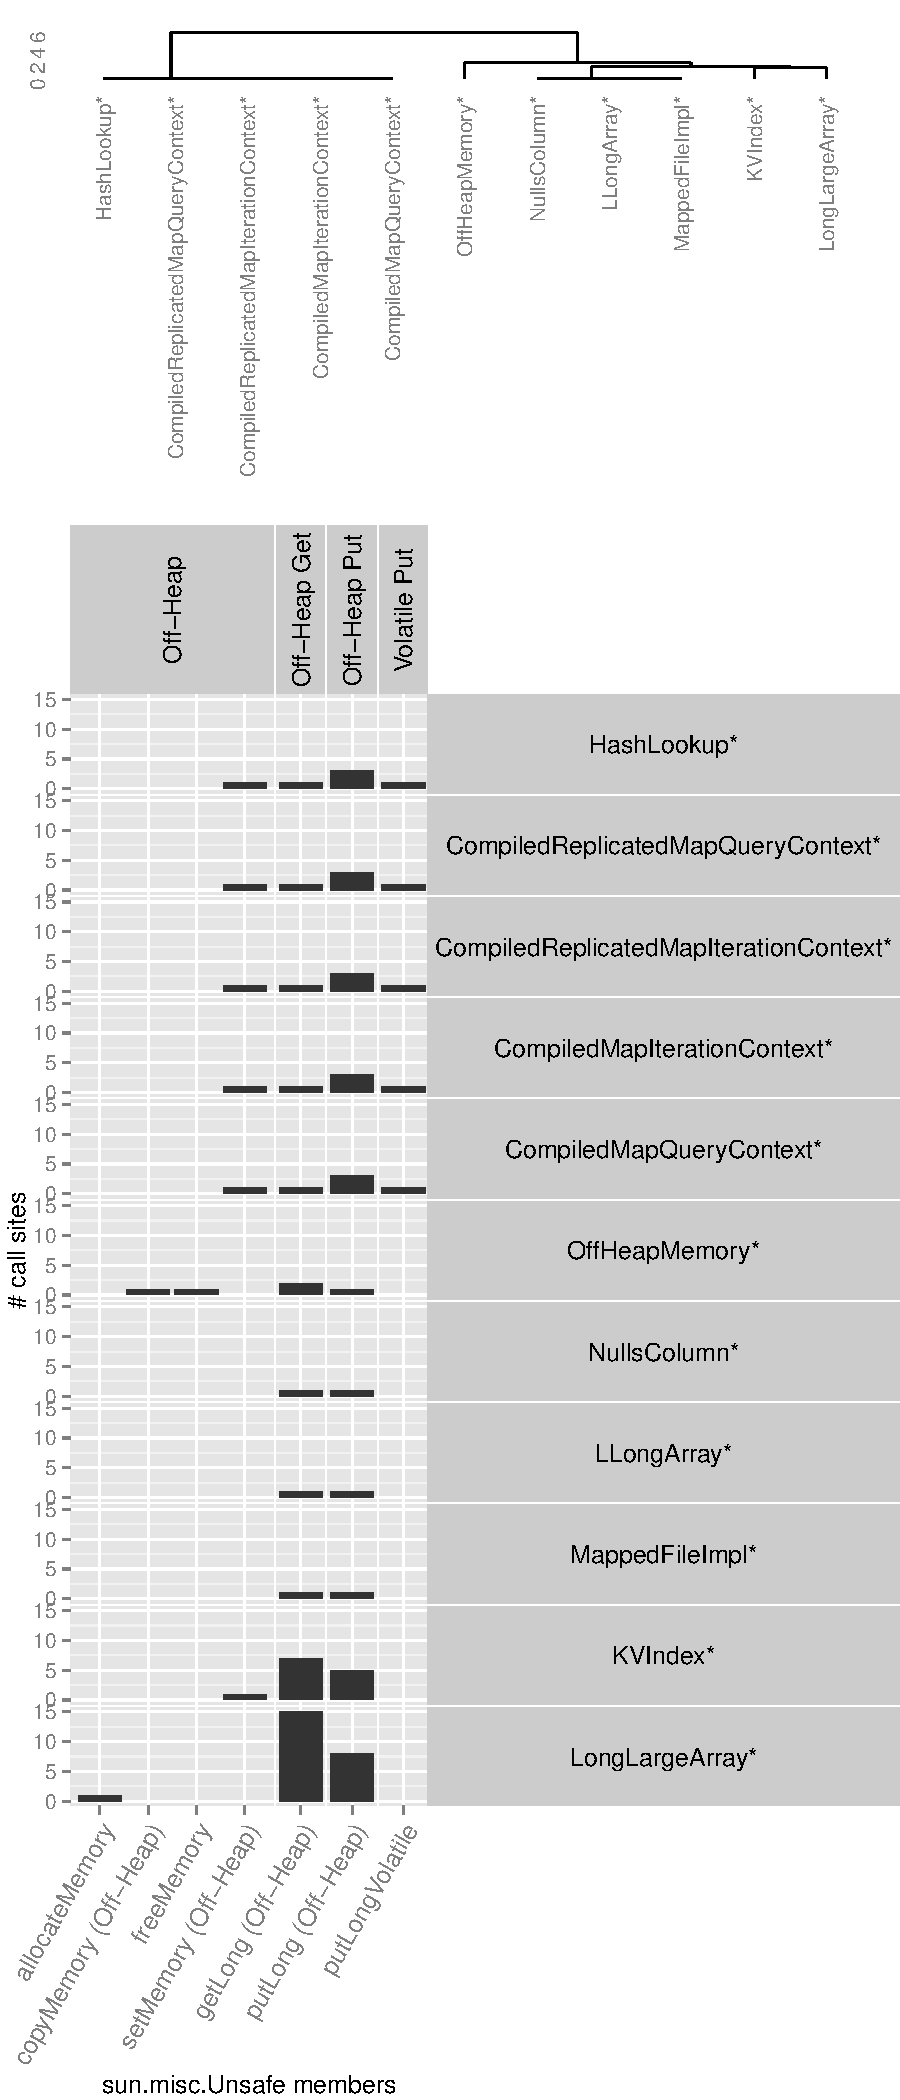
\includegraphics[width=\columnwidth]{chapters/unsafe/classunit}
\caption{Classes using off-heap large arrays}
\label{fig:classunitfingerprint}
\end{figure}

Once we had a clustering of the artifacts by method usage, we manually
inspected a sample of artifacts in each cluster to identify patterns.
Some artifacts contained more than one pattern.
For instance the cluster in Figure~\ref{fig:classunitfingerprint} contains
classes that use \unsafe{} to implement large off-heap arrays, but also
contains
calls to methods of the \smugroup{Put Volatile} group used to implement
strongly shared consistent variables.
We tagged each artifact manually inspected with the set of patterns that it exhibits.
%We have inspected each cluster by 
%--- of the most used artifacts ---


%\newcommand{\artitem}[3]{ \art{##1\}{##2\}{\} }

\newcommand{\sep}{

}
%\newcommand{\artitemurl}[4]{#1\footnote{#2}}
\newcommand{\artitem}[3]{\artexp{#2}{#3}}
%\newcommand{\artitemurl}[4]{\art{#2}{#3}{#4}}
\newcommand{\artitemurl}[4]{\artexp{#2}{#3}}
%\newcommand{\artitemurl}[4]{ ##1 ##2 ##3 \textbf{##4} }

\newenvironment{artlist}{}{}


\newcommand{\allocmost}{
\begin{artlist}
\artitemurl{springframework}{org.springframework}{spring-core}{http://projects.spring.io/spring-framework/}\sep{}
\artitemurl{objenesis}{org.objenesis}{objenesis}{http://objenesis.org/}\sep{}

\artitemurl{mockito}{org.mockito}{mockito-all}{https://github.com/mockito/mockito}
\end{artlist}
}

\newcommand{\probytemost}{
\begin{artlist}
\artitemurl{guava}{com.google.guava}{guava}{https://github.com/google/guava}\sep{}
\artitemurl{gwt-dev}{com.google.gwt}{gwt-dev}{http://www.gwtproject.org/}\sep{}

\artitemurl{lz4}{net.jpountz.lz4}{lz4}{https://code.google.com/p/lz4/}
\end{artlist}
}

\newcommand{\lockfreemost}{
\begin{artlist}
\artitemurl{scala-lang}{org.scala-lang}{scala-library}{http://scala-lang.org/}\sep{}
\artitemurl{apache-hadoop}{org.apache.hadoop}{hadoop-hdfs}{https://hadoop.apache.org/}\sep{}
\artitemurl{glassfish}{org.glassfish.grizzly}{grizzly-framework}{https://grizzly.java.net/}
\end{artlist}
}

\newcommand{\fencemost}{
\begin{artlist}
\artitem{scala-lang}{org.scala-lang}{scala-library}\sep{}

\artitemurl{jruby}{org.jruby}{jruby-core}{http://jruby.org/}\sep{}

\artitemurl{hazelcast}{com.hazelcast}{hazelcast-all}{http://hazelcast.com/}
\end{artlist}
}

\newcommand{\parkmost}{
\begin{artlist}
\artitem{scala-lang}{org.scala-lang}{scala-library}\sep{}

\artitemurl{jsr166}{org.codehaus.jsr166-mirror}{jsr166y}{http://xircles.codehaus.org/projects/jsr166-mirror}\sep{}

\artitemurl{netflix-servo}{com.netflix.servo}{servo-internal}{https://github.com/Netflix/servo}
\end{artlist}
}

\newcommand{\finalfieldmost}{
\begin{artlist}
\artitemurl{groovy}{org.codehaus.groovy}{groovy-all}{http://groovy-lang.org/}\sep{}
\artitemurl{jodd}{org.jodd}{jodd-core}{http://jodd.org/}\sep{}

\artitemurl{disruptor}{com.lmax}{disruptor}{http://lmax-exchange.github.io/disruptor/}
\end{artlist}
}

\newcommand{\monitormost}{
\begin{artlist}
\artitemurl{jboss}{org.jboss.modules}{jboss-modules}{http://www.jboss.org/}\sep{}
\artitemurl{cassandra}{org.apache.cassandra}{cassandra-all}{http://cassandra.apache.org/}\sep{}
\artitemurl{gridgain}{org.gridgain}{gridgain-core}{http://www.gridgain.com/}
\end{artlist}
}

\newcommand{\serializationmost}{
\begin{artlist}
\artitem{hazelcast}{com.hazelcast}{hazelcast-all}{}\sep{}
\artitemurl{kryo}{com.esotericsoftware.kryo}{kryo}{https://github.com/EsotericSoftware/kryo}\sep{}
\artitemurl{xstream}{com.thoughtworks.xstream}{xstream}{http://xstream.codehaus.org/}
\end{artlist}
}

\newcommand{\marshallingmost}{
\begin{artlist}
\artitemurl{eu.stratosphere}{eu.stratosphere}{stratosphere-core}{http://stratosphere.eu/}\sep{}

\artitemurl{jnr}{com.github.jnr}{jffi}{https://github.com/jnr/jffi}\sep{}

\artitemurl{jython}{org.python}{jython}{http://www.jython.org/}
\end{artlist}
}

\newcommand{\throwmost}{
\begin{artlist}
\artitemurl{io.netty}{io.netty}{netty-all}{http://netty.io/}\sep{}

\artitemurl{openhft}{net.openhft}{lang}{https://github.com/OpenHFT/Java-Lang}\sep{}

\artitemurl{ai.h20}{ai.h2o}{h2o-core}{https://github.com/h2oai/h2o-dev}
\end{artlist}
}

\newcommand{\sizemost}{
\begin{artlist}
\artitemurl{ehcache}{net.sf.ehcache}{ehcache}{http://ehcache.org/}\sep{}

\artitemurl{jamm}{com.github.jbellis}{jamm}{https://github.com/jbellis/jamm}\sep{}

\artitemurl{openjdk.jol}{org.openjdk.jol}{jol-core}{http://openjdk.java.net/projects/code-tools/jol/}
\end{artlist}
}

\newcommand{\largearraysmost}{
\begin{artlist}
\artitemurl{neo4j}{org.neo4j}{neo4j-primitive-collections}{http://neo4j.com/}\sep{}

\artitemurl{orientdb}{com.orientechnologies}{orientdb-core}{https://github.com/orientechnologies/orientdb}\sep{}

\artitemurl{mapdb}{org.mapdb}{mapdb}{http://www.mapdb.org/}
\end{artlist}
}

\newcommand{\pagemost}{
\begin{artlist}
\artitem{apache-hadoop}{org.apache.hadoop}{hadoop-common}{}\sep{}

\artitem{openhft}{net.openhft}{lang}\sep{}

\artitemurl{xerial}{org.xerial.larray}{larray-mmap}{https://github.com/xerial/larray}
\end{artlist}
}

\newcommand{\classmost}{
\begin{artlist}
\artitemurl{elasticserach}{org.elasticsearch}{elasticsearch}{https://github.com/elastic/elasticsearch}\sep{}

\artitemurl{mvel2}{org.apache.geronimo.ext.openejb}{core}{http://geronimo.apache.org/}\sep{}

\artitem{openhft}{net.openhft}{lang}
\end{artlist}
}


\newcommand{\javaclass}[1]{\emph{#1}}

\newcommand{\patternrow}[1]{
  \expandafter\newcommand\csname row#1\endcsname{\csname foundin#1\endcsname & \csname usedby#1\endcsname & \csname mostused#1\endcsname}
}

\newcommand{\patterntext}[6]{
    \expandafter\newcommand\csname desc#1\endcsname{#2}
    \expandafter\newcommand\csname alt#1\endcsname{#3}
    \expandafter\newcommand\csname impl#1\endcsname{#4}
    \expandafter\newcommand\csname rationale#1\endcsname{#5}
    \expandafter\newcommand\csname issues#1\endcsname{#6}
    \patternrow{#1}
}

\newcommand{\patternsection}[1]{

\expandafter\subsection{\csname name#1\endcsname}
\expandafter\label{sec:#1}

\noindent \textbf{\em Description.} \expandafter\csname desc#1\endcsname
%\smallskip

\noindent \textbf{\em Rationale.} \expandafter\csname rationale#1\endcsname
%\smallskip

\noindent \textbf{\em Implementation.} \expandafter\csname impl#1\endcsname
%\smallskip

\noindent \textbf{\em Issues.} \expandafter\csname issues#1\endcsname
%\smallskip

}

\newcommand\foundinalloc{88}
\newcommand\usedbyalloc{14794}
\newcommand\mostusedalloc{\allocmost}
\newcommand\membersalloc{\member{allocate\-Instance}}
\newcommand\namealloc{Allocate an Object without Invoking a Constructor}

\patterntext{alloc}%
{With this pattern an object can be allocated on the heap
without executing its constructor.}
{}
{The \member{allocate\-Instance} method takes as parameter a \javaclass{java.lang.Class} object, and returns a new instance of that class. Unlike allocating an
object directly, or through the reflection API, the object's constructor is not invoked.}
{This pattern is useful for creating mock objects for testing and in deserializing
serialized objects.}
{If the constructor is not invoked, the object might be left uninitialized
  and its invariants might not hold.
  Users of \member{allocate\-Instance} must take care to properly
  initialize the object before it is used by other code. This is often done in conjunction with other methods
  of \unsafe{}, for instance those in the \smugroup{Heap Put} group, or by using
the Java reflection API.
}

\newcommand\foundinprobyte{44}
\newcommand\usedbyprobyte{12274}
\newcommand\mostusedprobyte{\probytemost}
\newcommand\membersprobyte{\member{array\-Base\-Offset}, \member{getLong}, and optionally \member{array\-Index\-Scale} (to assert that the size of byte is equal to 1)}
\newcommand\nameprobyte{Process Byte Arrays in Block}

\patterntext{probyte}%
{When processing the elements of a byte array, better performance
can be achieved by processing the elements 8 bytes at a time, treating it as a
long array, rather than one byte at a time.}
{The JVM's runtime compiler can be extended with optimizations for vectorizing
byte array accesses.}
{The \member{array\-Base\-Offset} method is invoked to get the base offset of the byte array.
Then \member{getLong} is used to fetch and process 8 bytes of the array at a time.}
{The pattern is used for fast byte array processing, for instance,
when comparing two byte arrays lexicographically.}
{The pattern assumes that bytes in an array are stored contiguously. This may
  not be true for some VMs, \eg{} those implementing large arrays using
  discontinuous arrays or
  arraylets~\cite{siebertEliminatingExternalFragmentation2000,baconRealtimeGarbageCollector2003}. Users of
the pattern should be aware of the endianness of the underlying hardware.
In one \stackoverflow{} discussion, this pattern is
discouraged since it is non-portable and, on many JVMs, results in slower
code.\footnote{\url{http://stackoverflow.com/questions/12226123}} }

\newcommand\foundinlockfree{84}
\newcommand\usedbylockfree{10259}
\newcommand\mostusedlockfree{\lockfreemost}
\newcommand\memberslockfree{Either \member{object\-Field\-Offset} or \member{array\-Base\-Offset} in conjunction
  with \member{array\-Index\-Scale}, plus methods of the \smugroup{CAS} group
or the \smugroup{Fetch \& Add} group.
}
\newcommand\namelockfree{Atomic Operations}


\patterntext{lockfree}%
{
  To implement
  non-blocking concurrent data structures and synchronization primitives, hardware-specific atomic operations
  provided by \smu{} are used.
%Some of them include following classes developed by Cliff Click, author of
  %the HotSpot Server Compiler: \javaclass{ConcurrentAutoTable}, \javaclass{NonBlockingHashMap}.
%\javaclass{org.vmmagic}~\cite{Frampton:2009:DMH:1508293.1508305}.
}
{The Java standard library provides classes for some concurrent data structures.
The library also provides classes
(\javaclass{Atomic\-Field\-Reference\-Updater}, \javaclass{AtomicIntegerArray}, etc.)
for safely performing atomic operations on fields and array elements, as well
as several synchronizer classes. These
can be used instead of the \unsafe{} atomic operations.}
{To get the offset of a \java{} variable either \member{object\-Field\-Offset} or
  \member{array\-Base\-Offset}/\member{array\-Index\-Scale} can be used.
With this offset, the methods from the \smugroup{CAS} or \smugroup{Fetch \&
Add} groups are used to perform atomic operations on the variable.
Other methods of \unsafe{} are often used in the implementation of concurrent
data structures, including \smugroup{Volatile Get/Put}, \smugroup{Ordered Put}, and \smugroup{Fence} methods.
}
{Non-blocking algorithms often scale better than algorithms that use locking.}
{Non-blocking algorithms can be difficult to implement correctly. Programmers
must understand the Java memory model and how the \unsafe{} methods interact
with the memory model.}

\newcommand\foundinfence{198}
\newcommand\usedbyfence{9795}
\newcommand\mostusedfence{\fencemost}
\newcommand\membersfence{Methods of the \smugroup{Fence} group, or methods of
the \smugroup{Get/Put Volatile} groups or \smugroup{Put Ordered} group}
\newcommand\namefence{Strongly Consistent Shared Variables}


\patterntext{fence}%
{Because of Java's weak memory
  model, when implementing concurrent code,
  it is often necessary to ensure that
  writes to a shared variable by one thread become visible to other threads,
  or to prevent
  reordering of loads and stores.
  Volatile variables can be used for this purpose, but
  \smu{} can be used instead with better performance.
  Additionally, because Java does not allow array elements to be declared volatile,
  there is no possibility other than to use \unsafe{} to ensure visibility of
  array stores. The methods of the \smugroup{Ordered Put} groups
  and the \smugroup{Volatile Get/Put} groups can be used for these purposes.
  In addition, the \smugroup{Fence} methods were introduced in Java 8 expressly
to provide greater flexibility for this use case.}
{Memory fence operations can be added to the standard library. The language
can be changed to make volatile variables more flexible.}
{To ensure a write is visible to another thread, \smugroup{Volatile Put}
  methods or \smugroup{Ordered Put} methods can be used, even on non-volatile variables.
  Alternatively, a \member{storeFence} or \member{fullFence} can be used.
  \smugroup{Volatile Get} methods ensure other loads and stores are not reordered
  across the load. A \member{loadFence} could also be used before a read of a
  shared variable.
}{This pattern is useful for implementing concurrent algorithms or shared
  variables in concurrent settings. For instance, JRuby uses a \member{fullFence}
  to ensure visibility of writes to object fields.
}{Fences can replace volatile variables in some situations, offering better
  performance. Most of the uses of the pattern use the \smugroup{Ordered Put}
  and \smugroup{Volatile Put} methods. Since they were added to Java only recently, there are currently few instances
of the pattern that use the \smugroup{Fence} methods.}

\newcommand\foundinpark{62}
\newcommand\usedbypark{7330}
\newcommand\mostusedpark{\parkmost}
\newcommand\memberspark{\member{park}, \member{unpark}}
\newcommand\namepark{Park/Unpark Threads}


\patterntext{park}%
{The \member{park} and \member{unpark} methods are used to block and unblock threads and are useful for implementing locks and other
blocking synchronization constructs.}
{The standard library class \javaclass{java.\-util.\-concurrent.\-locks.\-LockSupport} provides \member{park} and \member{unpark}
methods to be used for implementing locks.}
{The \member{park} method blocks the current thread while \member{unpark}
unblocks a thread given as an argument.}
{The alternative to parking a thread is to busy-wait, which uses CPU
resources and does not allow other threads to proceed.}{Users of
  \member{park} must be careful to avoid deadlock.}

\newcommand\foundinfinalfield{11}
\newcommand\usedbyfinalfield{7281}
\newcommand\mostusedfinalfield{\finalfieldmost}
\newcommand\membersfinalfield{\member{object\-Field\-Offset}; and, at least one method of the \smugroup{Heap Put} or \smugroup{Put Volatile} groups.}
\newcommand\namefinalfield{Update Final Fields}

\patterntext{finalfield}%
{This pattern is used to update a final field.  }
{The reflection API can be used to implement the same functionality.}
{The \member{object\-Field\-Offset} methods and one of the \smugroup{Put} methods work in conjunction to directly modify the memory where a final field resides.}
{Although it is possible to use reflection to implement the same behavior,
  updating a final field is easier and more efficient using \smu{}.
  Some applications update final fields when cloning objects
  or when deserializing objects.
}{
  There are numerous security and safety issues with modifying final
  fields. The update should be done only on newly created objects
  (perhaps also using \member{allocate\-Instance} to avoid
  invoking the constructor) before the object becomes visible to
  other threads. The \java{} Language
  Specification (Section~17.5.3)~\cite{Gosling:2013:JLS:2462622}
  recommends that final fields not be read until all updates are
  complete. In addition, the language permits compiler optimizations
  with final fields that can prevent updates to the field from being
  observed.
  Since final fields can be cached by other threads, one instance of
  the pattern uses \member{putObject\-Volatile} to update the field rather than
  simply \member{putObject}.
  Using this method ensures that any cached copy in other threads
  is invalidated.}

\newcommand\foundinmonitor{14}
\newcommand\usedbymonitor{7015}
\newcommand\mostusedmonitor{\monitormost}
\newcommand\membersmonitor{\member{monitor\-Enter}, \member{monitor\-Exit}}
\newcommand\namemonitor{Non-Lexically-Scoped Monitors}

\patterntext{monitor}%
{In this pattern, monitors are explicitly acquired and released without using
\texttt{synchronized} blocks.}
{One can extend the language to support non-lexically-scoped
monitors.}
{One usage of the pattern is to temporarily release monitor locks acquired
  in client code (e.g., through a synchronized block or method) and
  then to reenter the monitor before returning
  to the client. The \member{monitor\-Exit} method is used to exit the
  synchronized block. Because monitors are reentrant, the pattern
  uses the method \javaclass{Thread.\-holds\-Lock} to implement a loop
  that repeatedly exits the monitor
  until the lock is no longer held. When reentering the monitor,
  \member{monitor\-Enter} is called the same number of times
  as \member{monitor\-Exit} was called to release the lock.
}{The pattern is used in some situations to avoid deadlock, releasing a monitor
temporarily, then reacquiring it.}{Care must be taken to balance calls to
\member{monitor\-Enter} and \member{monitor\-Exit}, or else the lock might
not be released or an \texttt{Illegal\-Monitor\-State\-Exception} might be
thrown.}

\newcommand\foundinserialization{32}
\newcommand\usedbyserialization{5689}
\newcommand\mostusedserialization{\serializationmost}
\newcommand\membersserialization{\member{object\-Field\-Offset} and methods of the \smugroup{Heap Get} and \smugroup{Heap Put} groups}
\newcommand\nameserialization{Serialization/Deserialization}

\patterntext{serialization}%
{In this pattern, \smu{} is used to persist and subsequently load objects to and from secondary memory dynamically.
Serialization in \java{} is so important that it has a \javaclass{Serializable} interface to automatically serialize objects that implement it.
Although this kind of serialization is easy to use, it does not offer good
performance and is inflexible.
It is possible to implement serialization using the reflection API. This is
also expensive in terms of performance. Therefore, fast serialization frameworks
often use \unsafe{} to get and set fields of objects.
% Project \project{jon} however invoke the \member{allocate\-Instance} method.
% These projects use one of the following classes:
% \javaclass{com.lts.xmlser.SerializationUtils},
% \javaclass{Sun14ReflectionProvider}, or
% \javaclass{JSX.magic.MagicClass14}, which are third-party classes that implement fast serialization.
Some of these projects use reflection to check if \smu{} is available, falling
back on a slower implementation if not.}
{Reflection can be used for accessing fields, more safely although less
  efficiently. Java's supports serialization of objects using
  \javaclass{java.io.Object\-Output\-Stream} and related classes. These serialization features could be extended with support for
user-defined serialization formats.}
{Methods of \smugroup{Heap Get} and \smugroup{Heap Put} are used to read and
  write fields and array elements. Deserialization may use
\member{allocate\-Instance} to create objects without invoking the constructor.}
{De/serialization requires reading and writing fields to save and restore
objects. Some of these fields may be final or private.}{
Using \unsafe{} for serialization and deserialization has many of the same issues
as using \unsafe{} for updating final fields (Section~\ref{sec:finalfield}) and for creating objects without
invoking a constructor (Section~\ref{sec:alloc}). Objects must not escape before being completely
deserialized. Type safety can be violated by using methods of the
\smugroup{Heap Put} group. In addition, care must be taken when deserializing
some data structures. For instance, data structures that use
\javaclass{System.identity\-Hash\-Code} or \javaclass{Object.hash\-Code} may need to rehash objects on
deserialization because the deserialized object might have a different
hash code than the original serialized object.}

\newcommand\foundinmarshalling{8}
\newcommand\usedbymarshalling{3690}
\newcommand\mostusedmarshalling{\marshallingmost}
\newcommand\membersmarshalling{Methods of the \smugroup{Off-Heap} and \smugroup{Off-Heap Get/Put} groups}
\newcommand\namemarshalling{Foreign Data Access and Object Marshaling}

\patterntext{marshalling}%
{In this pattern \smu{} is used to share data between Java code and code
  written in another language, usually C or C++.
% The \project{osfree} and \project{snarej} projects are peculiar because they use only \smugroup{Get} and \smugroup{Put} methods without calling \smugroup{Offset}.
% This is explained by the fact that these kinds of projects are implementing
% operating systems on top of the JVM.
% They obtain the memory address for the \smugroup{Get} and \smugroup{Put} methods using JNI.
% The \project{janux} project implements a native loader that needs to load class files from native memory.
% The \project{javapayload} project is about running exploits in pure \java{}, it has the ability to load a native library and execute an exploit.
% Stdlib: bytebuffer, datainputstream
}
{\javaclass{java.nio.Byte\-Buffer} and related classes can be used for marshaling data instead of \unsafe{}.}
{The methods of the \smugroup{Off-Heap} group are used to access memory off
the Java heap. Often a buffer is allocated using \member{allocate\-Memory},
which is then passed to the other language using JNI. Alternatively, the
native code can allocate a buffer in a JNI method. The \smugroup{Off-Heap Get}
and \smugroup{Off-Heap Put} methods are used to access the buffer.}{This
pattern is needed to efficiently pass data, especially structures and arrays, back and forth between Java and
native code. Using this pattern can be more efficient than using native
methods and JNI.}{Use of \unsafe{} here is inherently not type-safe. Care must be
  taken especially with native pointers, which are represented as
\texttt{long} values in Java code.}

\newcommand\foundinthrow{59}
\newcommand\usedbythrow{3566}
\newcommand\mostusedthrow{\throwmost}
\newcommand\membersthrow{\member{throw\-Exception}}
\newcommand\namethrow{Throw Checked Exceptions without Being Declared}

\patterntext{throw}%
{This pattern allows the programmer to throw checked exceptions without being
declared in the method's \texttt{throws} clause.}
{The issue can be avoided by not requiring \texttt{throws} declarations at
  all. Indeed, there is a long-running
  debate\footnote{\url{http://www.ibm.com/developerworks/library/j-jtp05254/}} about the
  software-engineering benefits of checked exceptions.
C\#, for instance, does not require that exceptions be declared in method signatures at all.
One alternative proposed in a \stackoverflow
discussion is to use Java generics
instead.\footnote{\url{http://stackoverflow.com/questions/11410042}} Because
of type erasure, a checked exception can be coerced unsafely into an unchecked exception and thrown.
}
{The pattern is implemented using the \member{throw\-Exception} method.}
{In testing and mocking frameworks, the pattern is used to circumvent declaring
  the exception to be thrown, which is often unknown.
It is used in the Java Fork/Join framework to save the generic exception of a thread to be re-thrown later.}
{This method can violate Java's subtyping
  relation, because it is not expected
  for a method that does not declare an exception to actually throw it. At
  run time, this can manifest as an uncaught exception.}

\newcommand\foundinsize{4}
\newcommand\usedbysize{3003}
\newcommand\mostusedsize{\sizemost}
\newcommand\memberssize{\member{array\-Base\-Offset}, \member{array\-Index\-Scale},
\member{object\-Field\-Offset}}
\newcommand\namesize{Get the Size of an Object or an Array}

\patterntext{size}%
{This pattern uses \smu{} to estimate the size of an object or an array in
memory.}
{A sizeof feature could be introduced into the language or
into the standard library to make the implementation portable.}
{To compute the size of an array, add \member{array\-Base\-Offset} and
\member{array\-Index\-Scale} (for the given array base type) times the array
length. For objects, use \member{object\-Field\-Offset} to compute the offset
of the last instance field. In both cases, a VM-dependent fudge factor is
added to account for the object header and for object alignment and padding.}{The object
size can be useful for making manual memory management decisions. For
instance, when implementing a cache, object sizes can be used to implement
code to limit the cache size.}{Object
size is very implementation dependent. Accounting for the object header and
alignment requires adding VM-dependent constants for these parameters.}

\newcommand\foundinlargearrays{12}
\newcommand\usedbylargearrays{487}
\newcommand\mostusedlargearrays{\largearraysmost}
\newcommand\memberslargearrays{\member{allocate\-Memory}, \member{free\-Memory}, \member{setMemory}, \member{getInt}, \member{getLong}, \member{putInt}, \member{putLong}}
\newcommand\namelargearrays{Large Arrays and Off-Heap Data Structures}

\patterntext{largearrays}%
{This pattern uses off-heap memory to create large arrays or data structures with manual memory management.}
{This functionality could be provided with a language feature or library.}
{A block of memory is allocated with \member{allocate\-Memory} and then
accessed using \smugroup{Off-Heap Get} and \smugroup{Off-Heap Put} methods.
The block is freed with \member{free\-Memory}.}
{Java's arrays are indexed by \texttt{int} and are thus limited to $2^{31}$
elements. Using \unsafe{}, larger buffers can be allocated outside the heap.}{This pattern has all the issues of manual memory
management: memory leaks, dangling pointers, double free, etc.
One issue, mentioned on
\stackoverflow, is that the memory returned by \member{allocate\-Memory} is
uninitialized and may contain
garbage.\footnote{\url{http://stackoverflow.com/questions/16723244}}
Therefore, care must be taken to initialize allocated memory before use.
The \unsafe{} method \member{set\-Memory} can be used for this purpose.
}

\newcommand\foundinpage{11}
\newcommand\usedbypage{359}
\newcommand\mostusedpage{\pagemost}
\newcommand\memberspage{\member{pageSize}}
\newcommand\namepage{Get Memory Page Size}


\patterntext{page}%
{\smu{} is used to determine the size of a page in memory.}
{This functionality could be added to the standard library, perhaps in
the \javaclass{java.nio} package.}
{Call \member{pageSize}.}{The page size is needed to allocate buffers or
  access memory by page.
  A common use case is to round up a buffer size,
  typically a \javaclass{java.nio.ByteBuffer}, to the
  nearest page size. Hadoop uses the page size to track memory usage of
  cache files mapped directly into memory
using \javaclass{java.nio.MappedByteBuffer}. Another use is to process a
buffer page-by-page.
Some native libraries require or recommend allocating buffers on page-size
boundaries.\footnote{\url{http://stackoverflow.com/questions/19047584}}
}{Some platforms on which the JVM runs do not have
  virtual memory, so requesting the page size is non-portable.
}

\newcommand\foundinclass{21}
\newcommand\usedbyclass{294}
\newcommand\mostusedclass{\classmost}
\newcommand\membersclass{\member{define\-Class}}
\newcommand\nameclass{Load Class without Security Checks}

\patterntext{class}%
{\smu{} is used to load a class from an array containing its bytecode. Unlike
with the \javaclass{ClassLoader} API, security checks are not performed.}
{This feature could be added to the standard library, with a
  \javaclass{SecurityManager} used to explicitly relax the Java security model.}
{The pattern is implemented using the \member{define\-Class} method, which
takes a byte array containing the bytecode of the class to load.}{This pattern is useful for implementing lambdas, dynamic
class generation, and dynamic class rewriting. It is also useful in application
frameworks that do not interact well with user-defined class loaders.}{The
pattern violates the Java security model. Untrusted code could be introduced
into the same protection domain as trusted code.}

\section{Usage Patterns of \smu{}}
\label{sec:unsafe:patterns}

This section presents the patterns we have found during our study.
We present them sorted by how many artifacts depend on them, as computed from
the Maven dependency graph described in Section~\ref{sec:unsafe:overview}.


% alloc probyte lockfree fence park finalfield monitor serialization marshalling throw size largearrays page class

A summary of the patterns is shown in Table~\ref{table:pats}.
The \textbf{\em Pattern} column indicates the name of the pattern.
\textbf{\em Found in}
indicates the number of artifacts in \mavencentral{} that contain the pattern.
\textbf{\em Used by}
indicates the number of artifacts that transitively depend on the artifacts with the
pattern.
\textbf{\em Most used artifacts}
presents the three most used artifacts containing the pattern, that is, the 
artifact with the most other artifacts that transitively depend upon it.
Artifacts are shown using their Maven identifier, \ie{}
\artexp{$\langle$groupId$\rangle$}{$\langle$artifactId$\rangle$}.
% \textbf{\em Members used}
% shows the members of \unsafe{} used in the pattern.

%\& \verb+\+textbf\{Unsafe members\}
\begin{table*}[t!]
\scriptsize
\centering
\caption{Patterns and their occurrences in the Maven Central repository}
\label{table:pats}
\begin{tabularx}{\linewidth}{rp{5.3cm}ccX}
\hdr    & \textbf{Pattern}              & \textbf{Found In} & \textbf{Used by} & \textbf{Most used artifacts} \\
\alt  1 & \namealloc                    & \rowalloc             \\
\row  2 & \nameprobyte                  & \rowprobyte           \\
\alt  3 & \namelockfree                 & \rowlockfree          \\
\row  4 & \namefence                    & \rowfence             \\
\alt  5 & \namepark                     & \rowpark              \\
\row  6 & \namefinalfield               & \rowfinalfield        \\
\alt  7 & \namemonitor                  & \rowmonitor           \\
\row  8 & \nameserialization            & \rowserialization     \\
\alt  9 & \namemarshalling              & \rowmarshalling       \\
\row 10 & \namethrow                    & \rowthrow             \\
\alt 11 & \namesize                     & \rowsize              \\
\row 12 & \namelargearrays              & \rowlargearrays       \\
\alt 13 & \namepage                     & \rowpage              \\
\row 14 & \nameclass                    & \rowclass             \\
\hline
\end{tabularx}
\end{table*}

We present each pattern using the following template.
\medskip

{

\noindent \textbf{\em Description.}
{What is the purpose of the pattern? What does it do?}
%\smallskip

\noindent \textbf{\em Rationale.}
{What problem is the pattern trying to solve? In what contexts is it used?}
%\smallskip

% \noindent \textbf{\em Unsafe members.}
% {Methods and fields of \smu{} used in the pattern.
% In some cases, there are multiple alternatives to implementing the pattern.
% These are explained when necessary in turn for each pattern. }
% %\smallskip

\noindent \textbf{\em Implementation.}
{How is the pattern implemented using \smu{}?}
%\smallskip

% \noindent \textbf{\em Found in.}
% {Number of artifacts in \mavencentral{} that contain the pattern.}
% %\smallskip

% \noindent \textbf{\em Used by.}
% {Number of artifacts that transitively depend on the artifacts with the
% pattern.}
% %\smallskip

% \noindent \textbf{\em Most used artifacts.}
% {The three most used artifacts containing the pattern, that is, the
% artifact with the most other artifacts that transitively depend upon it.
% Artifacts are shown using their Maven identifier, \ie{}
% \artexp{$\langle$groupId$\rangle$}{$\langle$artifactId$\rangle$}.
% %\smallskip

\noindent \textbf{\em Issues.}
{Issues to consider when using the pattern and problems discussed in the
\stackoverflow{} database.}
%\smallskip

% \noindent \textbf{\em Alternatives.}
% {Potential alternatives to using the \unsafe{} for solving the same
% problem.}


}



\patternsection{alloc}
\patternsection{probyte}
\patternsection{lockfree}
\patternsection{fence}
\patternsection{park}
\patternsection{finalfield}
\patternsection{monitor}
\patternsection{serialization}
\patternsection{marshalling}
\patternsection{throw}
\patternsection{size}
\patternsection{largearrays}
\patternsection{page}
\patternsection{class}


\section{What is the Unsafe API Used for?}
\label{sec:unsafe:discussion}

In response to \ref{unsafe:rq2} (\emph{\urqB}),
many of the patterns we found indicate that \unsafe{} is used to achieve 
better performance or to implement functionality not otherwise available in the \java{} language or standard library.

However, many of the patterns described can be implemented using APIs
already provided in the \java{} standard library. 
In addition, there are several existing proposals to improve the situation
with \unsafe{} already under development within the \java{} community.
Oracle software engineer Paul~\cite{psandoz14} performed a survey on
the OpenJDK mailing list to
study how Unsafe is
used\footnote{\url{http://www.infoq.com/news/2014/02/Unsafe-Survey}} and
describes several of these proposals.


% alloc probyte lockfree fence park finalfield monitor serialization marshalling throw size largearrays page class

\newcommand{\tick}{\cmark}
\newcommand{\exis}{$\bullet$}

\newcommand{\langalt}{\textbf{Lang}}
\newcommand{\opt}{\textbf{VM}}
\newcommand{\lib}{\textbf{Lib}}
\newcommand{\refl}{\textbf{Ref}}

% \newcommand{\hdr}{\rowcolor{header-color}}
% \newcommand{\alt}{\rowcolor{alt-row-color}}
% \newcommand{\row}{}
%\& \verb+\+textbf\{Unsafe members\}
\begin{table}[t!]
\centering
\caption{Patterns and their alternatives. A bullet (\exis) indicates that an
alternative exists in the \java{} language or API. A check mark (\tick) indicates that there is a proposed alternative for \java{}.}
\label{table:alts}
\begin{tabularx}{\linewidth}{rp{9.25cm}cccccccX}
\hdr \# & \textbf{Pattern}		& \langalt & \opt 	& \lib	& \refl	\\
\alt  1 & \namealloc    		& \tick	& 	& 	&	\\
\row  2 & \nameprobyte 			& 	& \tick	& 	&	\\
\alt  3 & \namelockfree			&	& 	& \exis	&	\\
\row  4 & \namefence 			& 	& 	& \tick &	\\
\alt  5 & \namepark			& 	& 	& \exis &	\\
\row  6 & \namefinalfield		& 	& 	& 	& \exis	\\
\alt  7 & \namemonitor			& \tick	& 	& 	&	\\
\row  8 & \nameserialization		& \tick & 	& \exis & \exis	\\
\alt  9 & \namemarshalling     		& \tick & 	& \exis	&	\\
\row 10 & \namethrow 			& \tick	& 	&   	&	\\
\alt 11 & \namesize 			& \tick	& 	& \tick &	\\
\row 12 & \namelargearrays 		& \tick & 	& \tick &	\\
\alt 13 & \namepage			& \tick	& 	& \tick	&	\\
\row 14 & \nameclass 			& \tick & 	& \tick	&	\\
\hline
\end{tabularx}
\end{table}


A summary of the patterns with existing and proposed alternatives to \unsafe{} is shown in Table~\ref{table:alts}.
The table consists of the following columns:
The \textbf{\em Pattern} column indicates the name of the pattern.
The next three columns indicate whether the pattern could be implemented either as a
language feature (\textbf{\em Lang}),
virtual machine extension (\textbf{\em VM}),
or
library extension (\textbf{\em Lib}).
The \textbf{\em Ref} column indicates that the pattern can be
implemented using reflection.
A bullet (\exis) indicates that an
alternative exists in the \java{} language or API. A check mark (\tick)
indicates that there is a proposed alternative for \java{}.

Many APIs already exist that provide functionality similar to \unsafe{}.
Indeed, these APIs are often implemented using \unsafe{} under the hood, but 
they are designed to be used safely.
They maintain invariants or perform runtime checks
to ensure that their use of \unsafe{} is safe.
Because of this overhead, using \unsafe{}
directly should in principle provide better performance at the cost of safety.
% We are unaware of any studies measuring this overhead, however.

For example,
the \javaclass{java.\-util.\-concurrent} package provides classes 
for safely performing atomic operations on fields and array elements, as well
as several synchronizer classes. These
classes
can be used instead of \unsafe{} to implement
atomic operations or strongly consistent
shared variables.
The standard library class
\javaclass{java.\-util.\-concurrent.\-locks.\-LockSupport} provides
\member{park} and \member{unpark}
methods to be used for implementing locks. 
These methods are just thin wrappers
around the \smu{} methods of the same name and 
could be used to implement the park pattern.
\java{} already supports serialization of objects using the
\javaclass{java.lang.Serializable} and
\javaclass{java.io.Object\-Output\-Stream} API.
The now-deleted JEP 187 Serialization 2.0 proposal%
\footnote{\url{http://mail.openjdk.java.net/pipermail/core-libs-dev/2014-January/024589.html}}
\footnote{\url{http://web.archive.org/web/20140702193924/http://openjdk.java.net/jeps/187}}
addresses some of the issues with \java{} serialization.

Because volatile variable accesses compile to code that issues memory fences, 
strongly consistent variables can be implemented by accessing volatile variables.
However, the fences generated for volatile variables may be stronger (and
therefore less performant) than are needed for a given application.
Indeed, the \unsafe{} \smugroup{Put Ordered}
and \smugroup{Fence} methods were likely introduced
to improve performance versus volatile variables.
% There is currently a proposal for enhanced volatile support in the JVM (JEP 193 Enhanced Volatiles~\cite{jep193}).
The accepted proposal JEP 193 (Enhanced Volatiles~\citep{jep193}) introduces \emph{variable handles}, which allow
atomic operations on fields and array elements.

Many of the patterns can be implemented using the reflection API,
albeit with lower performance than with \unsafe{}~\citep{korlandNoninvasiveConcurrencyJava2010}.
For example,
reflection can be used for accessing object fields to implement serialization.
Similarly, reflection can be used
in combination with
\javaclass{java.nio.Byte\-Buffer} and related classes for
data marshaling.
The reflection API can also be used to write to final fields.
However, this feature of the reflection API 
makes sense only during deserialization or during object construction and may have
unpredictable behavior in other cases.

% \footnote{\url{http://docs.oracle.com/javase/8/docs/api/java/lang/reflect/Field.html\#set(java.lang.Object,\%20java.lang.Object)}}

Writing a final field through reflection may not ensure
the write becomes visible to other threads that might have cached the final
field, and it may not work correctly at all if the VM performs compiler
optimizations such as constant propagation on final fields.

Many patterns use \unsafe{} to use memory more efficiently.
Using \code{struct}s or packed objects can reduce memory overhead by eliminating object headers and other per-object overhead.
\java{} has no native support for \code{struct}s,
but they can be implemented with byte buffers or with \jni{}.\footnote{\url{http://www.oracle.com/technetwork/java/jvmls2013sciam-2013525.pdf}}

The Arrays 2.0 proposal~\citep{arrays20} and
the value types proposal~\citep{valuetypes} address the large arrays pattern.
Project Sumatra~\citep{layouts} proposes features for accessing GPUs
and other accelerators,
one of the use cases for foreign data access.
Related proposals include JEP 191~\citep{jep191},
which proposes a new foreign function interface for \java{},
and Project Panama~\citep{panama}, which supports native data access from the \jvm{}.

A \member{sizeof} feature could be introduced into the language or into the standard library.
A use case for this feature includes cache management implementations.
A higher-level alternative might be to provide an \api{} for memory usage tracking in the \jvm{}.
A page size method could be added to the standard library,
perhaps in the \javaclass{java.nio} package,
which already includes \javaclass{MappedByteBuffer} to access memory-mapped storage.

Other patterns may require \java{} language changes.
For instance, 
the language could be changed to not require methods to declare the exceptions they throw,
obviating the need for \unsafe{} in this case.
Indeed, there is a long-running debate\footnote{\url{http://www.ibm.com/developerworks/library/j-jtp05254/}} about the software-engineering benefits of checked exceptions.
C\#, for instance, does not require that exceptions be declared in method signatures at all.
One alternative not requiring a language change
% , proposed in a \stackoverflow{} discussion,
is to use \java{} generics
instead.
% \footnote{\url{http://stackoverflow.com/questions/11410042}}
Because of type erasure, a checked exception can be coerced unsafely into an unchecked exception and thrown.

Changing the language to support allocation without constructors or non-lexically-scoped monitors is feasible.
However, implementation of these
features must be done carefully to ensure object invariants
are properly maintained.
In particular, supporting arbitrary unconstructed
objects can require type system changes to prevent usage of the object 
before initialization~\citep{qiMaskedTypesSound2009}.
Limiting the scope of this feature to support deserialization only may be a good compromise and
has been suggested in the JEP 187 Serialization 2.0 proposal.

Since \unsafe{} is often used simply for performance reasons,
virtual machine optimizations can reduce the need for \unsafe{}.
For example, the \jvm{}'s runtime compiler can be extended with optimizations for vectorizing byte array accesses,
eliminating the motivation to use \unsafe{} to process byte arrays.
Many patterns use \unsafe{} to use memory more efficiently.
This could be ameliorated with lower GC overhead.
There are proposals for this, for instance JEP 189 Shenandoah:
Low Pause GC~\citep{jep189}.

\section{Conclusions}
\label{sec:unsafe:conclusions}

\smu{} is an API that was designed for limited use in system-level runtime library code.
The \unsafe{} API is powerful, but dangerous.
The improper use of \unsafe{} undermines \java{}'s safety guarantees.
We studied to what degree \unsafe{} usage has spread into third-party libraries,
to what degree such third-party usage of \unsafe{} can impact existing Java code,
and which \unsafe{} API features such third-party libraries actually use.
We studied the questions and discussions developers have about \unsafe{},
and we identified common usage patterns.
We thereby provided a basis for evolving the \unsafe{} API, the \java{} language, and the \jvm{}
by eliminating unused or abused unsafe features,
and by providing safer alternatives for features that are used in meaningful ways.
We hope this will help to make \unsafe{} safer.